%
% Szakdolgozatminta az Eszterházy Károly Katolikus Egyetem
% matematika illetve informatika szakos hallgatóinak.
%

\documentclass[
% opciók nélkül: egyoldalas nyomtatás, elektronikus verzió
% twoside,     % kétoldalas nyomtatás
% tocnopagenum,% oldalszámozás a tartalomjegyzék után kezdődik
]{thesis-ekf}
\usepackage[T1]{fontenc}
\PassOptionsToPackage{defaults=hu-min}{magyar.ldf}
\usepackage[magyar]{babel}
\usepackage{mathtools,amssymb,amsthm,pdfpages}
\footnotestyle{rule=fourth}

\usepackage{listings}
\renewcommand{\lstlistingname}{}

\newtheorem{tetel}{Tétel}[chapter]
\theoremstyle{definition}
\newtheorem{definicio}[tetel]{Definíció}
\theoremstyle{remark}
\newtheorem{megjegyzes}[tetel]{Megjegyzés}

\lstdefinelanguage{TypeScript}{
	language=Java,
	morekeywords={await, async, let, const, type, interface},
	sensitive=true
}

\lstset{
	language=TypeScript,
	basicstyle=\ttfamily\small,
	keywordstyle=\color{blue}\bfseries,
	commentstyle=\color{green},
	stringstyle=\color{red},
	numbers=left,
	numberstyle=\tiny\color{black},
	stepnumber=1,
	breaklines=true,
	frame=single,
	backgroundcolor=\color{lightgray},
	xleftmargin=2.5cm,
	xrightmargin=2.5cm,
	framexleftmargin=5mm,
	framexrightmargin=5mm 
}

\begin{document}

\institute{Matematikai és Informatikai Intézet}
\title{Mesterséges intelligencia számítógépes játékokban}
\author{Budai Roland\\Programtervező informatikus BSc.}
\supervisor{Dr. Kovásznai Gergely\\Egyetemi docens}
\city{Eger}
\date{2024}
\maketitle

\tableofcontents

\chapter*{Bevezetés}
\addcontentsline{toc}{chapter}{Bevezetés}

A szakdolgozatom témája egy stratégiai társasjáték implementálása beépített Mesterséges intelligenciával, amely segít a támadási döntések meghozatalában. A projekt ötlete nem csupán egy tanulmányi kötelezettség teljesítéséből fakad, hanem egy régebb óta tervezett hobbi projekt része is. Már a tanulmányaim elején megfogalmazódott bennem a kérdés, hogy hogyan tudnék egy hasonló társasjátékot a számítógépes világban megvalósítani. Milyen adatbázist kell elkészíteni, milyen döntéseket hozhatnak a játékosok, hogyan lehet megoldani, hogy egyszerre többen is hozzáférjenek az adatokhoz, mégis konzisztens maradjon a játékmenet és a tárolt állapotai a játéknak? Hasonló kérdések fogalmazódtak meg bennem tanulmányaim során, melyekre a képzés ideje alatt egyre jobb és jobb ötleteket sikerült szereznem. Mindezek miatt nagy lelkesedéssel álltam neki a feladatnak a témaválasztást követően. 

További érdekessége a szakdolgozatnak a mesterséges intelligencia (MI) fejlesztése, használata. A mesterséges intelligencia és a gépi tanulás területei egyre nagyobb szerepet játszanak a modern játékfejlesztésben, ezért ez a projekt nemcsak szakmai kihívást jelentett számomra, hanem egyben kiváló lehetőséget is arra, hogy mélyebben megismerkedjek az MI alkalmazásával, fejlesztésével a játékok világában. Az MI implementálásával lehetőségem nyílt egy olyan ellenfél létrehozására, amely képes tanulni és folyamatosan fejlődni a játékok során. 

A mesterséges intelligencia fejlődése az elmúlt években jelentősen befolyásolta a játékfejlesztés folyamatát, lehetővé téve, hogy az MI-alapú ellenfelek egyre intelligensebb döntéseket hozzanak és alkalmazkodjanak a játékosok stratégiájához. Stratégiai döntések meghozatalához különösen a projektemben is használt megerősítéses tanulás (reinforcement learning, RL) vált népszerűvé, amely az MI folyamatos fejlődését, tanulását teszi lehetővé.

A szakdolgozatomban szeretnék elsősorban a mesterséges intelligenciáról írni, bemutatni a projektet általánosságban, hogy milyen technológiák kerültek felhasználásra. Ezek után magáról a játékról, annak szabályairól lesz szó, majd ennek a konkrét implementációjáról online környezetben. Részletesen kifejtem a mesterséges intelligencia megtervezésének és fejlesztésének folyamatát, majd végezetül bemutatom az elkészült alkalmazást, összefoglalom a fejlesztés során szerzett tapasztalatokat. A projekt a következő GitHub linken érhető el: \url{https://github.com/Rolidroid0/Szakdolgozat}.

\chapter{MI és technológia}

\section{A gépi tanulás elméleti alapjai és a megerősítéses tanulás}

A mesterséges intelligencia fejlődése során a gépi tanulás (machine learning, ML) kapott kiemelkedő szerepet az intelligens rendszerek fejlesztésében. A gépi tanulás olyan módszereket foglal magában, amelyek lehetővé teszik a számítógépes modellek számára, hogy tapasztalatok alapján javítsák a teljesítményüket, a programozásuk ember általi megváltoztatása nélkül. Az ML három fő típusa a felügyelt tanulás (supervised learning), a felügyelet nélküli tanulás (unsupervised learning) és a megerősítéses tanulás. \cite{ML}

A felügyelt tanulás esetében a rendszer egy előre meghatározott bemenet-kimenet párokból álló adathalmazon tanul, míg a felügyelet nélküli tanulás során a modell mintázatokat keres egy struktúra nélküli adathalmazon belül. Ezekkel szemben a megerősítéses tanulás egy olyan módszer, amelyben egy ügynök (agent) a környezetével (environment) interakcióba lépve tanul, és az akciókért visszacsatolást kap jutalmak (reward) vagy büntetések formájában.

\subsection{Neurális hálózatok}

A neurális hálózatok az ML egy legfontosabb eszközei, amelyek a biológiai neuronhálózatok mintájára épülnek fel. Egy mély neurális hálózat (deep neural network, DNN) több rétegű csomópontokból áll, ahol az egyes rétegek között súlyok segítségével történik az információátadás. Ezek az architektúrák jól alkalmazhatók képfelismerés, természetes nyelvfeldolgozás és komplex döntéshozatali folyamatok esetén. A megerősítéses tanulásban gyakran alkalmaznak mély neurális hálózatokat, például Deep Q-Network algoritmust, amely egy Q-tanulási (Q-learning) stratégiát kombinál mély tanulási modellekkel, lehetővé téve az ügynök számára a nagyobb állapottérrel rendelkező környezetben való hatékony tanulást. \cite{NN}

\subsection{Az ügynök és a környezet fogalma}

Egy megerősítéses tanulást alkalmazó szoftver fejlesztése során két központi elemet kell meghatároznunk: az ügynököt és a környezetet. Az ügynök az a döntéshozó entitás, amely egy adott állapotban kiválaszt egy akciót a környezet befolyásolására. A környezet pedig az a rendszer, amelyben az ügynök működik. Folyamatosan visszacsatolást ad az ügynök döntéseire jutalmak vagy büntetések formájában. A tanulási folyamat során az ügynök folyamatosan próbálja maximalizálni az összegyűjtött jutalmat, miközben az ismeretlen környezetben kísérletezik és tanul a visszajelzések alapján.

\subsection{Megerősítéses tanulás}

Mint említettem, a megerősítéses tanulás (Reinforcement Learning, RL) olyan gépi tanulási módszer, amelyben az ügynök egy környezetben interakciók során tanul optimális stratégiákat kialakítani. Az RL egyik legfőbb célja a döntéshozatal optimalizálása egy adott probléma keretein belül. \cite{RL} A megerősítéses tanulás egyik alapvető fogalma az állapot (state, $S$), amely a környezet aktuális reprezentációja, amely leírja az ügynök és a környezet közötti pillanatnyi helyzetet. A cselekvés (action, $A$) az ügynök által végrehajtható lépések halmaza. A jutalom (reward, $R$) a környezet visszacsatolása egy adott cselekvés végrehajtása után. Az ügynök célja ezen jutalom hosszú távon való maximalizálása. Az ügynök által használt politika (policy, $\pi$) egy szabályrendszer, amely meghatározza, hogy egy adott állapotban milyen cselekvést hajtson végre az ügynök. A hosszú távú jutalom várható értékének számításához egy adott állapot és cselekvés kombinációját használja, ez az úgynevezett Q-érték (Q-value, $Q(s,a)$).

Az RL során az ügynök kísérlet és hiba (trial and error) folyamat révén tanulja meg a várhatóan legjobb kimenetelű döntéseket. Számtalan algoritmust használhatunk a tanításhoz, ezek közül a legismertebbek közé tartozik a Q-learning és a Deep Q Nerwork (DQN), amelyek az állapot-cselekvés értékek (Q-értékek) becslésén alapulnak.

A megerősítéses tanulás alkalmazásai számos területet lefednek, beleértve a robotikát, az önvezető járműveket és a stratégiai játékokat. Egy stratégiai játékban az RL lehetőséget ad arra, hogy a mesterséges intelligencia adaptálódjon a játékos döntéseihez, és folyamatosan fejlessze saját taktikáját. Az ilyen típusú modellek egyik legfontosabb előnye, hogy nem előre megírt szabályok szerint működnek, hanem a tapasztalatokból tanulnak és fejlődnek.

\section{Felhasznált technológiák}

A projekt megvalósítása során több különböző technológiát alkalmaztam, amelyek lehetővé tették a játék és a mesterséges intelligencia hatékony implementálását. Az MI fejlesztésének alapját a Python nyelv képezte, mivel számos hatékony könyvtár áll rendelkezésre a gépi tanulás számára. A neurális hálózat betanításához és optimalizálásához a PyTorch keretrendszer nyújtott megoldást. A játék backendjének fejlesztéséhez JavaScript-et alkalmaztam, amely lehetővé tette a szerveroldali logikák és az adatkezelés megvalósítását. Az adatokat a dokumentumorientált MongoDB adatbázisban tároltam. A React szolgált egy dinamikus és interaktív frontend fejlesztésére. A szerver és a különböző kliensek közötti kommunikációt kétféleképpen oldottam meg. Az alapvető adatok lekérdezésére REST API-n keresztüli kommunikációt biztosítottam, a valós idejű játékélmény és gyors adatcsere érdekében pedig WebSocket kapcsolatot hoztam létre. További fejlesztési eszközként szolgáltak a GitHub, a Visual Studio Code és az Inkscape amely a frontendhez szükséges svg kiterjesztésű fájlok létrehozásában segített.

\chapter{Játékmechanika}

Ebben a fejezetben bemutatom a játék alapvető mechanikáit, szabályrendszerét, valamint a játékosok interakcióit és a játékmenet fázisait. A játék egy körökre osztott stratégiai társasjáték digitális implementációja, amelyben a játékosok különböző területek felett próbálnak uralmat szerezni, harcolnak egymással, és erőforrásokat kezelnek. A játék szabályrendszere, mechanikái és karakterei a játék készítőinek\footnote{Hasbro} szellemi termékei, és ezen elemek kidolgozása nem az én saját alkotásom, csak tanulási célból alkalmazom őket a dolgozatom során.

\section{A játék szabályrendszere és célja}

A játékot többféleképpen lehet játszani, kettő játékostól egészen hétig, egy vagy két térkép bevonásával. A különböző játékmódok különböző bónuszokat tartalmaznak, mint a karakterkártyák, a pénz és erődítmények. A végső implementációmban a legegyszerűbb kétszemélyes játékváltozat lett megvalósítva, ezért a továbbiakban ennek a szabályait fogom részletezni. 

A játék célja, hogy a játékosok előre meghatározott győzelmi feltételt teljesítsenek, amely lehet bizonyos pontszám elérése, vagy az összes többi játékos legyőzése. A játékosok egy-egy házat képviselnek, és a térképen található területek felett próbálnak uralmat szerezni támadások és stratégiai döntések révén. 

A játéktér egy rácsszerkezetként értelmezhető térkép, amely különböző régiókra oszlik. Minden régió több területet tartalmaz, amelyek birtoklása kulcsszerepet játszik a játékosok stratégiájának kialakításában. A területek rendelkezhetnek erődökkel és kikötőkkel, amelyek befolyásolhatják a harci döntéseket. A játék legelején véletlenszerűen kiosztásra kerül 12-12 terület a két játékos között, majd a maradék területeket az úgynevezett semleges seregek birtokolják. Minden területre a játékosok felhelyeznek két sereget, majd a területkártyák megkeverésre kerülnek úgy, hogy a játék vége kártya a pakli alsó felébe kerüljön véletlenszerű helyre.

Egy játékos körében négy különböző akciót lehet végrehajtani: erősítés, invázió, manőver és húzás. A játék szabályai biztosítják, hogy minden játékos azonos eséllyel induljon, és a stratégiai döntéseik határozzák meg a végeredményt. A körökre osztott rendszer lehetővé teszi, hogy a játékosok átgondolják lépéseiket és reagáljanak az ellenfeleik akcióira.

Amikor a pakliba rejtett játék vége kártya a felszínre kerül, minden játékos megszámolja a pontjait és a legtöbb ponttal rendelkező játékos nyer. Pont jár a területek, a várak és a kikötők birtoklásáért. Természetesen ha egy játékos minden területet megszerez, automatikusan megnyeri a játékot.

\section{Játékosok interakciói és fázisai}

A játékosok interakciói alapvetően három fő dolgon alapszanak: területfoglalás, csaták és diplomácia. Mint említettem a játék egy körökre osztott rendszerben zajlik, ahol a körök több fázisból állnak. Minden kör végén a következő játékos veszi át az irányítást. A négy fázis/végrehajtható akció a következő:

\begin{itemize}
	\item \textbf{Erősítés}: a játékos minden köre elején plusz seregeket kap, amelyekkel tetszőlegesen erősítheti a birtokában lévő területeket. A plusz seregek számát a következőképpen számolják:
	\begin{itemize}
		\item A birtokolt területek számát össze kell adni a rajtuk lévő várak számával, elosztani hárommal és lefelé kerekíteni. Fontos kiegészítés, hogy legalább három sereget mindenképpen kap a játékos, még ha a számolás eredményeképp kevesebb járna is.
		\item Minden terület egy régióhoz tartozik és minden régiónak van egy plusz seregeket jelentő értéke. Ha egy játékos egy adott régió összes területével rendelkezik, akkor a meghatározott plusz seregeket hozzáadhatja az eddigi erősítésként járó seregeihez. Természetesen ha több régiót is teljesen birtokol egy játékos, akkor az összes régió bónuszt megkapja.
		\item Minden területkártyán van egy különleges egységet ábrázoló kép, amelyekből ha három összegyűlik további seregekre tehet szert a játékos. Fontos megjegyzés, hogy nem lehet öt kártyánál többet birtokolni, ha ebben a fázisban öt kártyája van egy játékosnak, azokból mindenképpen be kell váltania hármat. További bónusz seregekre tehet szert a játékos, ha a beváltott kártyákon lévő területeket is birtokolja. Ilyenkor két extra sereget helyezhet fel kizárólag ezekre a területekre.
		%TODO: ide bevágni a területkártyás táblázatot?
	\end{itemize}
	Végezetül az összes meghatározott plusz sereget el kell helyezni a táblán a játékos által birtokolt területekre. Ezeket lehet tetszőlegesen elosztani vagy akár mindet egy területre lehelyezni.
	\item \textbf{Inváziók és csaták}: Az inváziók és csaták a játék és a játékos körének a legfontosabb eseményei. Itt kell eldönteni, hogy kit és hol támadnak meg a játékosok, ezáltal közelebb kerülve a győzelemhez. Egy körben bármennyi inváziót kezdeményezhet a játékos, azonban egy területről csak egy támadás indítható adott körben. Olyan területeket lehet támadni, amelyek szomszédosak a kezdeményező területtel és ellenség birtokolja őket. A kikötővel rendelkező területek szomszédosnak számítanak egymással, ezáltal ezekről a területekről akár messzebbre is el lehet kezdeni terjeszkedni. Természetesen a játékos bármennyiszer támadhat egy körben amennyiszer lehetséges, de akár dönthet úgy is, hogy egyszer sem támad, ekkor automatikusan folytatódik a kör a következő fázissal. Egy invázió megkezdésekor ki kell választani, hogy melyik területről és melyik területre szeretne támadni a játékos, továbbá meg kell határoznia a támadó seregek számát. Ez a szám nem haladhatja meg az adott területen lévő seregeinek a számát és legalább egy sereget hátul kell hagynia, hogy ne maradjon üresen a terület. Miután egy invázió sikeresen létrejön, megkezdődnek a csaták. A támadó fél maximum három sereggel csatázhat, még ha ennél többel is kezdte meg az inváziót, és a védekező pedig legfeljebb két sereggel védekezik. Mindkét játékos a csatázó seregeinek számával megegyező kockával dob, majd ezeket az értékeket párosítják a legmagasabbaktól a legalacsonyabbakig. Ha a támadó legnagyobb dobása a magasabb, akkor a védekező veszít egy sereget, ha a védekező dobása a nagyobb vagy egyenlő, akkor pedig a támadó vesz le egy sereget. Hasonló összehasonlítás történik a második legnagyobb dobásokkal is. Ha az egyik fél több kockával dobott, aminek nem jutott már párja, akkor azt figyelmen kívül kell hagyni, az nem okoz veszteséget egyik fél számára sem. Ez egészen addig ismétlődik, amíg az egyik fél seregei el nem fogynak az adott invázió során. Ekkor ha a védőnek nem marad serege a megtámadott területen, a támadó megszerzi az adott területet, és a megmaradó seregei felkerülnek erre a területre. A semleges seregek által birtokolt területekre hasonló szabályok érvényesek, viszont a dobásokat nem a másik játékos végzi, hanem azok automatikusan végrehajtódnak.
	\item \textbf{Manőver}: Amikor a játékos úgy dönt, hogy nem támad tovább ebben a körben, akkor egyszer megteheti, hogy a seregei mozgatásával megerősít egy területet. Az átcsoportosítás során tetszőleges számú sereget (egy seregnek mindenképpen maradnia kell a területen) helyez át egy területről egy másik, azzal összeköttetésben lévő területre. Két terület akkor áll összeköttetésben, ha a köztük lévő összes terület ugyan azé a játékosé, tehát ellenséges vagy semleges területeken nem mozoghat át sereg.
	\item \textbf{Területkártyák húzása}: Végezetül a játékos köre végén ha legalább egy ellenséges területet meghódított, húzhat egy területkártyát a pakli tetejéről. Egy körben csak egyet húzhatnak a játékosok, függetlenül a megszerzett területek számától. A megszerzett kártyákat az erősítés részben tárgyalt módon lehet plusz seregekre váltani.
\end{itemize}

\chapter{Implementáció}

\section{Fejlesztési környezet és eszközök}

A projekt fejlesztéséhez Visual Studio Code-ot használok, mivel támogatja mind a Javascript, TypeScript és Python nyelveket, továbbá különböző bővítményekkel egyszerűsíthető a fejlesztési folyamat. Egy ilyen bővítmény például a MongoDB, ami által könnyedén ellenőrizhetjük az adatbázisban történő változások sikerességét. A verziókövetésre a GitHub szolgál, amely lehetővé teszi a változások követését és a biztonságos tárolást, így felváltva tudom fejleszteni a projektet asztali számítógépről és laptopról.

\subsection{Backend}

A játék alapját egy Node.js alapú backend biztosítja, amely a MongoDB adatbázissal kommunikálva tárolja és frissíti a különböző játékállapotokat. A szerver Express.js keretrendszert használ a HTTP és WebSocket kapcsolatok kezelésére, lehetővé téve a valós idejű kommunikációt a játékosok között. A backend struktúrája a következő mappákra oszlik: models, routes, constrollers, services, utils, handlers, config és db-seed. 

A \emph{models} mappában az adatbázisban tárolt dokumentumok sémái találhatók, mint például a kártyák vagy területek modellei. Ezen modellek felhasználásával történik meg az adatbázis feltöltése is a \emph{db-seed} mappában elhelyezkedő fájlok segítségével. 

A \emph{routes} az API végpontok definiálására szolgál, amelyek a kliens kéréseit kezelik. Ezekhez a végpontokhoz tartoznak különböző műveletek, amelyek a \emph{controllers} mappában helyezkednek el. Az üzleti logika nagy része itt történik, a kérések itt kerülnek feldolgozásra. A controller-ek különböző szolgáltatásokat használnak, akár többet is, amelyek a \emph{services} mappában találhatók. Ezek az önállóan működő szolgáltatások a legfontosabbak, hiszen ezeken keresztül történik a kommunikáció az adatbázissal. A különböző játékbeli lépések itt vannak rendszerezve egy-egy fájlban, mint például a \emph{cardsService.ts}, amely a kártyákhoz tartozó függvényeket tartalmazza (kártyák keverése, kártya húzása, kártyák beváltása seregekre). Azok a függvények, amelyek különféle segédfüggvények, például adatellenőrzések és egyéb általános műveletek az \emph{utils} mappában helyezkednek el.

A \emph{config} mappában két lényeges része kerül beállításra a szervernek: az adatbázissal való kapcsolat és a WebSocket szerver. Az adatbázishoz való csatlakozás egy Singleton osztály, amely ha nincs még csatlakozva egy mongoose.Connection példányon keresztül, akkor kialakít egy kapcsolatot az adatbázis URI-ját használva. A WebSocket szerver pedig létrehozza a szervert, majd várja a kliensek fel- és lecsatlakozását, illetve az üzeneteiket. Minden üzenetnek tartalmaznia kell egy kívánt akciót és opcionális adatokat. Az akciók a \emph{handlers} mappában kerülnek feldolgozásra a neveik alapján. Mindhez tartozik egy függvény, amelyek a különböző szolgáltatásokat hívják meg az akciók végrehajtására, majd visszajelzést küldenek az üzenetet küldő kliensnek, vagy bizonyos esetekben az összes kliensnek (például egy terület megerősítéséről minden kliensnek tudnia kell, lásd:~\ref{wss-clients}).

\lstinputlisting[caption={WSS kliensek értesítése.}, label=wss-clients, captionpos=b]{wssClients.ts} 

\subsection{Frontend}

A React segítségével épített frontend biztosítja a játékosok számára az interaktív felületet egy webes alkalmazás formájában. A React könyvtár komponens alapú felhasználói felületek létrehozására alkalmas. Az egész alapját az App.tsx fájl adja, amely a főoldalnak felel meg. Ezen helyezkednek el a különböző komponensek, mint például a fejléc. Az egyes komponensek két részből állnak, egy tsx fájlból, amely tartalmazza a hozzá tartozó mezőket és függvényeket, illetve a végén egy HTML szerű leírást és egy css fájlból, ami pedig a formázásban és megjelenítésben segít. A legtöbb komponens rendelkezik egy UseEffect() függvénnyel, amely folyamatosan figyeli, hogy érkezik-e üzenet a szerver felől WebSocket-en keresztül, ha igen, akkor pedig a tartalma alapján eldönti, hogy módosítania kell-e valamit a mezőin, vagy nem neki szólt ez az üzenet. A szerverhez hasonlóan a klienseken is fut egy szolgáltatás, amely egy Singleton osztálynak felel meg, és ezáltal csatlakozik a WebSocket szerverhez. Ebben a szolgáltatásban tudnak regisztrálni a komponensek úgynevezett handler-eket, amelyek figyelik a szervertől kapott üzenetek tartalmát. További szolgáltatások is megtalálhatók a kliensek kódjában, ezek azonban az API végpontok elérésében segédkeznek. Szintén a szerverhez hasonlóan itt is megjelennek az egyes adatbázis entitások modelljei. 

A frontend egyik legkiemelkedőbb része a térkép. Ez az \emph{assets} mappában helyezkedik el egy svg fájlként, amelyet az Inkscape program használatával került megalkotásra. Minden terület egyedi azonosítóval rendelkezik, amely a játékbeli névvel egyezik meg, így a frontend felismerheti őket. A ReactSVG könyvtár biztosítja az interaktivitást, lehetővé téve az elemek manipulációját. Például egy területre való kattintásnál az a terület élesebb színűvé válik, illetve az azonosító alapján meg tud nyílni oldalt a hozzá tartozó fül a terület adataival. Továbbá minden területen számszerűen megjelenik a rajta elhelyezkedő seregek száma a birtokos házának színével. 

%TODO: kép a térképről, úgy, hogy az egyik területre rá van kattintva 

\section{Adatkezelés és játékállapot tárolása}

A játék egyik legfontosabb eleme a játékállapot pontos eltárolása, amely biztosítja a játékosok számára a legfrissebb helyzeteket. Ezáltal az adatbázis tervezése volt az egyik legfontosabb feladat az implementáció során. 

A projektben MongoDB-t használok, mivel ez egy NoSQL-alapú, dokumentum-orientált adatbázis. JSON-szerű dokumentumokat használ, amik könnyedén lekérdezhetők, kezelhetők és bővíthetők, ezáltal jól illeszkednek a játékstruktúrához. \cite{MongoDB} A játékállapot folyamatos frissítése során fontos biztosítani, hogy ne történjenek ütközések, illetve adatvesztések. Ennek biztosítására kínál lehetőséget a MongoDB az Atomic Update műveletekkel, mint például az updateOne() és findOneAndUpdate() beépített függvények.

\lstinputlisting[caption={Példa az Atomic Update műveletekre a cardsService.ts-ből.}, label=kod-atomic-update, captionpos=b]{atomicUpdate.ts}

Hat adatbázis-kollekció lett létrehozva, a következőképpen (lásd: \ref{collections}~ábra):

\begin{figure}[ht!]
	\centering
	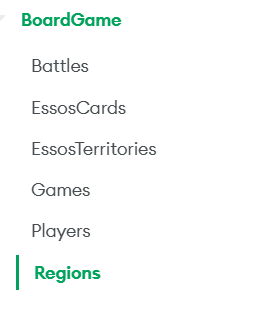
\includegraphics[width=5cm]{Collections.png}
	\caption{A MongoDB-ben tárolt kollekciók.}
	\label{collections}
\end{figure}

\begin{itemize}
	\item \textbf{Players}: a játékosok adatait tartalmazza
	\item \textbf{Games}: az aktuális és lezárt játszmák állapotát tartalmazza
	\item \textbf{EssosTerritories}: a térkép területeit és kapcsolataikat írja le
	\item \textbf{EssosCards}: a játékban szereplő kártyák helyzetét rögzíti
	\item \textbf{Regions}: a területeket összekötő régiókat tartalmazza
	\item \textbf{Battles}: a folyamatban lévő és lezárt csaták részleteit kezeli
\end{itemize}

A játék adatbázisának célja, hogy hatékonyan kezelje a játékállapotot, a területek, a játékosokat, a kártyákat és a csatákat. Az alábbiakban részletesen bemutatom az egyes táblák szerepét, a közöttük lévő kapcsolatokat, valamint az adatok kezelésének menetét. A régiókat tartalmazó kollekció a Regions.csv-ből került betöltésre, azonban mivel ezek az adatok nem változnak játék közben és két játék között sem, ezért ezzel a táblával adatmódosítás szempontjából nem is kell foglalkozni. Fő célja a kör elején kapott bónusz seregek számításánál a régióbónusz meghatározása. Erre a calculatePlusArmies(playerId: ObjectId) metódusban kerül sor (ahogy az \aref{region-bonus} kódrészletben látható).

\lstinputlisting[caption={Régióbónusz meghatározása.}, label=region-bonus, captionpos=b]{regionBonus.ts}

Egy új játék elkezdésénél elsősorban a Games kollekció került módosításra. A state mezője felel a játék státuszának követésében, háromféle értéket vehet fel: ongoing, azaz ez a játék még éppen folyamatban van, terminated, miszerint a játék valamilyen oknál fogva befejeződött, le lett zárva a szerver által és X won, ahol az X a győztes játékos házának neve. Amikor valaki elindít egy új játékot, akkor a szerver megnézi, hogy van-e folyamatban lévő játék, és ha van, akkor azt lezárja, majd létrehoz egy új példányt egyedi azonosítóval és a kört 1-re állítja.

Ezután következik a kártyák betöltése a seedEssosCards() függvénnyel és ezek megkeverése a shuffle() függvénnyel. Hasonlóan a régiókhoz, a kártyák is egy csv-ből kerülnek az adatbázisba, azonban a kártyák minden játék elején újratöltődnek. Minden kártyánál beállításra kerül a játékazonosító mező az előtte létrehozott új játék azonosítójával, illetve a tulajdonos mező "in deck" azaz a pakliban értéket vesz fel. A shuffle() biztosítja, hogy a kártyák véletlenszerűen legyenek elhelyezve a pakliban (a játék vége kártya is itt van biztosítva, hogy ne kerülhessen elő túl hamar, lásd \ref{game-end-card}~ábra).

\lstinputlisting[caption={A játék vége kártya helyének biztosítása.}, label=game-end-card, captionpos=b]{GameEndCard.ts}

Miután minden kártya a helyére került, a generatePlayers(numberOfPlayers: number) függvény kerül meghívásra. A függvény létrehozza a kívánt mennyiségű játékost és betölti őket az adatbázisba, majd a Games kollekcióban módosításra kerül a players tömb, belekerülnek az újonnan létrehozott játékosok házainak nevei.

Végezetül a területek kerülnek az adatbázisba a seedEssosTerritories() függvénnyel. A függvény csak betölti a területekhez tartozó általános adatokat, az allocateTerritories() függvény felel a terület birtokosának meghatározásában. Ez a függvény két játékos között osztja szét a területeket a következőképpen: 12 véletlenszerűen választott területet kap az első játékos, 12 területet a második és a maradék terület birtokosa a semleges értéket kapja. Mindezek után az első játékos megkapja a neki járó plusz seregeket és kezdődhet is a játék.

Egyetlen kollekció van, amely egy új játék létrehozásánál nem játszik semmilyen szerepet, a csatákat tartalmazó tábla. Ez a kollekció felel a már lejátszott és a még zajló csaták nyomon követésében. Amikor egy csata létrejön, akkor beállításra kerülnek az alapvető mezők mint például a támadó azonosítója, vagy a védekező terület azonosítója a szerver által. A csata közben a kör száma mező módosul, a dobások értékeinek mezője, illetve a csatanapló. Ha egy csatának vége van, akkor az állapota módosul az egyik fél győzelmére, majd a csatanaplóban lehet visszanézni, hogy pontosan hogyan is ment végbe az adott csata.

\begin{figure}[ht!]
	\centering
	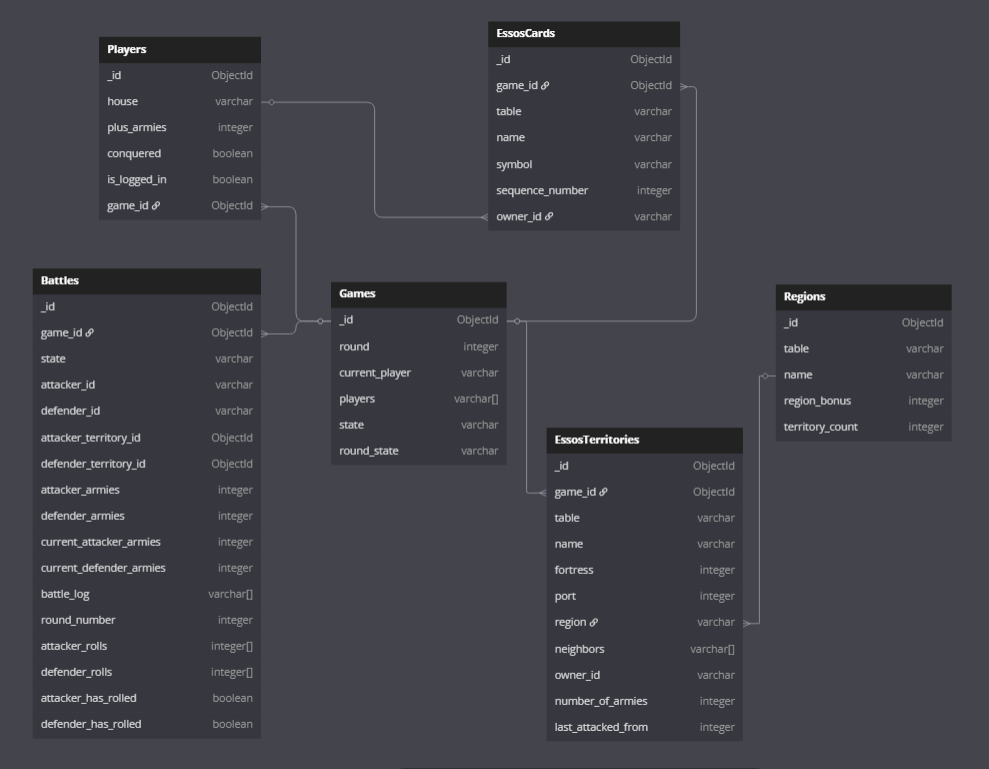
\includegraphics[width=16cm]{DB.png}
	\caption{Az adatbázis teljes tervezete.}
	\label{database}
\end{figure}

%TODO: adatbázis képet beletenni és hivatkozni rá + a 3.2-es kódrészletre is 

\chapter{Mesterséges intelligencia tervezése}

A mesterséges intelligencia integrálása a játékba egy összetett folyamat, amely több különböző lépést igényel. Az MI feladata a játékomban olyan stratégiai döntéseket biztosítani a játékos számára az invázió fázis folyamán, amelyek hosszútávon segítenek a játék megnyerésében. A fejlesztés során több szempontot is figyelembe kellett venni, mint például a szerverrel történő kommunikációt, a környezet megfelelő modellezését, illetve az ügynök és neurális hálózat fejlesztését.

\section{A neurális hálózat és az ügynök}

Az egyik legfontosabb lépés a megfelelő könyvtár/keretrendszer kiválasztása az ügynök és a neurális hálózat számára. Ezekre már többféle megoldás létezik, a kutatásom során ezek közül kettőt néztem meg mélyebben: a TensorFlow.js-t és a PyTorch-ot.

A TensorFlow.js egy olyan gépi tanulásos könyvtár, ami JavaScript nyelven alapul. A segítségével futtathatunk meglévő modelleket, újra taníthatjuk őket, vagy akár írhatunk sajátokat is JavaScript használatával. A meglévő modelleket futtathatjuk webes, illetve böngészőalapú alkalmazásainkban és Node.js környezetben különböző feladatok megoldásához. Ilyen feladatok például a képosztályozás, arc- és tárgyfelismerés vagy különböző nyelvi kérdések megválaszolása. Ezek által kiváló megoldást jelenthet webalapú játékok esetén is. Meglévő modell újratanítása a társasjátékom esetében nem volt opció, mivel a megerősítéses tanuláson alapuló modellek általában specifikus feladatokhoz készülnek, ezért egy meglévő modell alkalmazása a játékomban nem feltétlenül eredményes. A különböző játékokban eltérő környezetekkel és döntési struktúrákkal találkozunk, amelyek miatt egy előre betanított modell aligha illeszkedne jól a játékom szabályaihoz. A TensorFlow.js-en belüli Reinforcement Learning használata meglehetősen bonyolult lenne, mivel jelenleg nem érhető el kifejezetten az RL-nek dedikált könyvtár, mint például a Python-alapú TensorFlow tf-agents csomagja. A TensorFlow.js lehetővé teszi a gépi tanulási modellek JavaScript-ben való használatát, azonban RL specifikus implementációkat nem biztosít. \cite{TFJS}

A PyTorch egy nyílt forráskódú gépi tanulási keretrendszer, amelyet elsősorban a Facebook AI Research (FAIR) fejlesztett ki. A PyTorch népszerűsége főként a dinamikus számítási gráfoknak, a könnyen használható API-nak és a hatékony GPU-gyorsításnak köszönhető. Az egyszerű szintaxis és a rugalmas modellépítési lehetőségek miatt különösen kedvelt a kutatók és fejlesztők körében. A PyTorch támogatja a mély neurális hálózatok különböző architektúráit, és lehetőséget biztosít a modell tanítására, validálására és kiértékelésére. A megerősítéses tanulás területén a PyTorch egyik legnagyobb előnye, hogy kompatibilis több RL-keretrendszerrel, például a Stable-Baselines3-mal és az RLlib-bel, amelyek már előre implementált algoritmusokat tartalmaznak. Emellett elérhető a TorchRL környvtár, amely kifejezetten megerősítéses tanulási modellek fejlesztésére készült, és támogatja a legnépszerűbb algoritmusokat, mint a DQN. \cite{PYTCH}

Általánosan egy megerősítéses tanulást alkalmazó keretrendszer olyan ügynököket használ, amelyek célja egy virtuális környezetben való optimalizált döntéshozás. A döntéshozatal mellett tanulnak az elvégzett akciók és a velük járó jutalmak közötti kapcsolatokból, ezáltal fejlesztve a jövőbeli optimális döntéshozatalukat. Az ügynökök többféle módszert alkalmazhatnak, például: DQN, REINFORCE, DDPG, TD3, PPO, SAC.

\subsection{Folyamatos és diszkrét akciótér}

A megfelelő ügynök kiválasztása előtt meg kell vizsgálni egy fontos kérdést. A gépi tanulásban fontos fogalmak a diszkrét, illetve folytonos akcióterek. \cite{ActSpac} Ezek nem mást, mint a döntési lehetőségek típusát jelzik. Egy diszkrét akciótérben (discrete action space) az ügynök egy véges, meghatározott számú akció közül választhat, például mozoghat jobbra, balra, fel vagy le egy rácson. Jól alkalmazható olyan játékoknál, ahol a lépések száma korlátozott, mint a sakknál. A folytonos akciótérben (continuous action space) az ügynök tetszőleges, folytonos értékeket választhat egy adott tartományban, például gyorsulási fokot vagy kormányzási szöget egy autós szimulációban. Az én játékomat tekintve az ügynök meghatározott lehetőséggel rendelkezik: kiválaszthatja, hogy melyik területre helyez seregeket, honnan támad és mennyi sereggel, stb. Míg a sereg mennyiségének kiválasztása közelíthet a folytonos akciótérhez, a lépések száma és jellege jól leírható diszkrét döntési lehetőségekkel, így feltehetőleg a diszkrét módszerek (például DQN vagy PPO) megfelelőek lesznek.

\subsection{DQN és PPO}

Mind a DQN (Deep Q-Network - Mély Q-Hálózat), és a Q-tanulás a megerősítéses tanulás módszerei közé tartozik. A Q-tanulás egy algoritmus, ahol az ügynök rendel egy úgynevezett Q-értéket minden lehetséges állapot-akció pároshoz. Minden lépésnél az algoritmus frissíti ezeket az értékeket annak alapján, hogy az adott akcióért milyen jutalmat kapott. A cél az, hogy az ügynök a lehető legjobb, azaz a legnagyobb Q-értékkel rendelkező akciót válassza, ezáltal optimalizálva a hosszútávú döntéseit. A Q-tanulás segítségével az ügynök lépésről lépésre, iteratívan fejleszti a meghozott döntéseit, amíg el nem éri a maximális értékű (optimális) stratégiájának kifejlesztését. Ezen gondolatot kiegészítve, a DQN továbbfejleszti a hagyományos Q-tanulást mély neurális hálózatok alkalmazásával. Míg egy Q-tanulást alkalmazó ügynök táblázatot használ az egyes állapot-akció párok Q-értékeinek tárolására, a DQN egy mély neurális hálózatot használ a Q-függvény megközelítésére. Ezáltal az ügynöknek lehetősége nyílik olyan komplexebb környezetekben is hatékonyan tanulni, ahol egyébként a lehetséges állapotok száma túl nagy lenne egy hagyományos Q-tanulás táblázatos megoldásának. A DQN tanulási folyamata során az ügynök folyamatosan frissíti a neurális hálózatának súlyait annak érdekében, hogy minél pontosabban megjósolja az egyes akciók hosszú távú jutalmát. Kijelenthetjük, hogy mindkét módszer célja az ügynöknek egy optimális döntéshozó képesség kifejlesztése, azonban a DQN ideálisabb megoldást nyújt egy komplex, sok állapottal rendelkező környezetben. Mivel a DQN mély neurális hálózatot használ a Q-értékek kiszámításához, azaz nem kell minden egyes állapot-akció párról egyedi adatot tárolni, ezért egy hatékonyabb, skálázhatóbb megoldást jelent.

A többi ügynököt vizsgálva még a PPO (Proximal Policy Optimization) eshet számításba, ugyanis a többi a folytonos akcióterekben nyújt megoldást. A PPO Policy-alapú tanulást alkalmaz, úgynevezett policy-kat (döntési szabályokat) fejleszt. Ezek a policy-k megmondják az ügynöknek, hogy milyen lépést válasszon az adott helyzetben. Célja, hogy egy stabil, könnyen beállítható módszert biztosítson a tanuláshoz, korlátozva a policy változásának mértékét, így megelőzve a gyakori, instabil lépésváltozásokat. Eme korlátozás eléréséhez az úgynevezett "clipping" mechanizmust alkalmazza, amely biztosítja, hogy a policy frissítése ne legyen túl nagy egy adott irányban. Ha a változás mértéke meghalad egy bizonyos küszöböt, a klip hatására a policy frissítés elutasítja az optimális szintet meghaladó változásokat így megakadályozva a túltanulást, instabilitást. \cite{PPO}

\section{Kommunikáció a szerverrel}

Mivel a szerverem JavaScript nyelven íródott, illetve az MI Python nyelven kerül megvalósításra, valahogyan meg kell oldanom, hogy a kettő tudjon kommunikálni egymással. Az egyik megoldás a Python alkalmazáson belül egy REST API létrehozása (például Flask keretrendszerrel), ahol a Node.js szerver HTTP-kéréseket küldene, és a Python API pedig visszaadná az eredményeket. Ezzel a megoldással az a probléma, hogy nem valós idejű kommunikációra optimalizált. Ezzel szemben hatékonyabb megoldást nyújt a WesSocket kapcsolat. A Python és a Node.js között egy kétirányú, valós idejű kommunikációt biztosíthatunk a segítségével. Ez egy aszinkron adatcserét eredményez, ami hosszabb adatok küldésére és fogadására a legoptimálisabb. A Python oldalon hasonlóan a kliensekhez a WebSocket kapcsolat úgy van megoldva, hogy csatlakozik a szerverhez a Python kliens. A frontend kliensekkel ellentétben azonban a Python kliens minden kérésnél hozzáad egy random generált request\_id-t, amelyet a szerver figyelembe vesz. Ez azért fontos, mivel a Python részen nem szükséges megkapni minden üzenetet, amit a szerver folyamatosan küldözget például egy új játék létrehozásánál. Ezzel a megoldással a Python kliens egy olyan üzenetre vár, ami tartalmazza a kérése azonosítóját, és csak akkor megy tovább, amikor a megfelelő választ megkapta. \ref{python-client-awaiting}

\lstinputlisting[caption={Python kliens várakozása a megfelelő válaszra.}, label=python-client-awaiting, captionpos=b]{PythonClientAwaiting.py}

Végül a játék mesterséges intelligenciájának működéséhez egy FastAPI-alapú szerver is fut, amely fogadja a kliens kéréseit és visszaadja az AI által választott akciót. Ez a frontend kliensek miatt került bele a játékba, hogy tudják kérni az eddig betanított AI segítségét. A szerver a uvicorn segítségével futtatható, amely egy aszinkron webkiszolgáló Pythonhoz, és különösen jól működik az async és await alapú alkalmazásokkal. A FastAPI segítségével egy REST API készült, amely egy /predict/ végpontot biztosít. Ez a végpont fogad egy JSON formátumú kérést, amely tartalmazza a játék állapotát és a lehetséges akciókat. Az API először a bemeneti adatokat egy megfelelő formátumba alakítja (\_flatten\_state függvény), majd meghívja az  ügynököt, amely a tanult modell alapján kiválasztja a legjobb akciót. A választott akciót az API visszaküldi a kliensnek, így a játék képes az MI döntései alapján továbbhaladni.

\section{Környezet tervezése}
\label{környezet-tervezése}

A mesterséges intelligencia döntéshozatali folyamatainak tanításához elengedhetetlen egy jó környezet, amelyből tanulhat. Ennek a környezetnek pontosan kell szimulálnia a játék adott mechanizmusát, különben az MI rossz mintákat tanul meg, amelyek a valódi játékban irrelevánsnak számíthatnak. Ezért egy egyedi megvalósítást kellett megalkotni, amely pontosan követi a játék lépéseit, szabályait. A Gym nevezetű könyvtárat használtam fel kiindulási alapnak, amely lehetővé teszi az egyedi megerősítéses tanulás környezetek kialakítását. A Gym-en belül is az Env osztályt írtam felül, amely alapjáraton a következő függvényeket tartalmazza: init, step, reset és render. 

Az \emph{init} függvényben a környezet legfontosabb mezői kapnak értéket. Az egyik ilyen a megfigyelési tér (Observation Space), amely a játék aktuális állapotát modellezi. Az MI a döntéshozatalhoz öt információt használ. Az ownership, amely a területek birtoklását jelenti, értéke lehet 1, ha az AI birtokolja és 0, ha egy ellenfele. Az army\_counts, amely az egyes területeken lévő seregeket reprezentálja. Értéke az adott területen lévő seregek száma osztva egy maximum értékkel. Az attackable mutatja, hogy mely területek azok, amelyekről az AI indíthat támadást jelen pillanatban. Az utolsó két értékek pedig az is\_my\_turn és a round\_state, amelyekkel ellenőrizhető, hogy valóban az AI támadási köre van jelenleg. Másik fontos mező amely értéket kap az akciótér (Action Space), amely a végrehajtható akciókat tartalmazza dinamikusan. Ezek az akciók minden lépés után a get\_valid\_attacks() függvénnyel (\ref{get-valid-attacks}) kerülnek meghatározásra. Ezeknek a maximuma a területek száma szorozva a területek száma mínusz eggyel, szorozva a maximális seregekkel, majd a végén plusz egy, a passzolási lehetőség miatt. 

\lstinputlisting[caption={Akciótér beállítása.}, label=get-valid-attacks, captionpos=b]{GetValidAttacks.py}

A \emph{reset} függvény felel a környezet újrakezdéséért, minden lejátszott játék után ez a függvény kerül meghívásra a tanítás során. A WebSocket-en keresztül küld a szervernek egy új játék kezdése kérést, majd a válasz alapján beállítja a kezdéshez szükséges adatokat. A legnagyobb különbség az egyes állapotok lekérése és a legelső állapot lekérése között az a statikus adatok beállítása. Ilyen adatok a kikötők és várak elhelyezkedése a területeken, vagy a szomszédsági mátrix (egy \emph{n}x\emph{n}-es mátrix, ahol az \emph{n} a területek száma, a mátrix értékei pedig azt jelzik, hogy a két terület szomszédos-e), ugyanis ezek nem változnak a játék folyamán.

A \emph{step} az egyetlen függvény, amely egy paramétert is vár. A paraméter a választott akció sorszáma, amelyet kikeres a környezet az elérhető akciókból. Miután ellenőrizte, hogy valóban a kör helyes szakaszában van és a lépés is létezik, megnézi, hogy a választott lépés a passzolás-e. Ha igen, akkor az automata-kör kérést küldi a szervernek, ha pedig nem, akkor egy csata-kezdése kérést küld, csatolva a támadó és védekező területek azonosítóját, a játékos azonosítóját és a seregek számát. Mindkét esetben egy jutalom értéket vár vissza a szervertől, amely ha meghalad egy bizonyos értéket, akkor befejezettnek tekinti az adott játékot. Ha ez az érték nem elég nagy, azaz még folyamatban van a játék, akkor pedig a jutalom értéke mellett a következő állapotot is visszaadja az MI-nek. Amikor egy automata-kör kérés érkezik a szerver számára, akkor a seregek lehelyezése egy algoritmus alapján megy végig, csak egyesével lepakolja őket a területekre sorban. Az ellenfél köre pedig szintén egy egyszerű algoritmus alapján szimulálódik le: megnézi a birtokolt területeket, azok közül is azokat, amelyek rendelkeznek ellenséges szomszéddal, majd megnézi hogy ezen a területen van-e elég sereg a biztonságos támadáshoz. Csak akkor támad, ha legalább három serege van, és ha a saját seregek száma legalább kétszer annyi, mint a védekezőé. A támadó seregek számát úgy választja meg, hogy a támadók száma a maximum sereg felének felel meg, de legalább kettő kell, hogy legyen, de nem támadhat annyi sereggel, hogy csak egy maradjon a területen. Ha az így kiválasztott seregek száma nagyobb, mint a védekező seregek száma, akkor támadást indít. Ha egy támadás elindul, vagy nem talál egy megfelelőt sem, akkor az algoritmus leáll és visszatér, majd újra az MI következik. Magyarán csak akkor támad, ha biztos fölénye van, és igyekszik minimalizálni a kockázatot.

A \emph{render} valójában a környezet vizuális megjelenítéséért lenne felelős, azonban a játékomhoz már létezik frontend a kliensek számára, ezért az a függvény nem került implementálásra a környezeten belül.

\section{Tanítás és fejlesztés}

Az inváziók eldöntésére létrehozott mesterséges intelligenciát tehát egy mély Q-hálózat alapú tanulóalgoritmus irányítja, amely megerősítéses tanulást tartalmaz. A rendszer egy neurális hálózatot használ, amely tapasztalatokból tanul, egy replay buffer segítségével. A fejlesztés során a tanulási folyamat több komponensre oszlik: a környezet (és annak interfészei), a tanuló ügynök, valamint a mély Q-hálózat. Mindezt pedig egy train.py fájlban összesítem egy DQNTrainer osztályban.

\textbf{Környezet (Environment)}: A tanulási folyamat egy játékbeli szimulált környezetben történik, amelyet az AttackEnvironment osztály definiál (Bővebben lásd:~\ref{környezet-tervezése}.~fejezet). Ez az osztály biztosítja a környezet interakcióit, az elérhető akciók listáját, valamint a környezet visszacsatolásait (jutalmakat).

\textbf{DQN ügynök (DQNAgent)}: A tanulás kulcseleme a DQNAgent osztály, amely az alábbiakat kezeli:

\begin{itemize}
	\item \textbf{Akció kiválasztása}: Az epsilon-greedy stratégiát alkalmazza, hogy az ügynök kezdetben véletlenszerű akciókat válasszon, majd idővel egyre inkább a tapasztalatokra alapozott döntéseket hozzon.
	\item \textbf{Tapasztalatok tárolása}: A tanuláshoz szükséges múltbeli tapasztalatokat egy replay bufferben tárolja.
	\item \textbf{Tanulási folyamat}: A Q-értékeket folyamatosan frissíti a célhálózattal való kontraszt alapján.
	\item \textbf{Célhálózat frissítése}: Fenntart egy állandóan frissített célhálózatot, amely a tanulás stabilitását biztosítja.
	\item \textbf{Modell mentése és betöltése}: A betanított modellt egy pth formátumú fájlban tárolja, amelyet bármikor be lehet tölteni, hogy az eddigi tapasztalatokat tovább lehessen tanítani, vagy csak a döntését kérni.
\end{itemize}

\textbf{Mély Q-Hálózat (DeepQNetwork)}: A DQN alapja egy mély neuronhálózat, amelyet a DeepQNetwork osztály valósít meg. A hálózat egy bemeneti rétegből, két rejtett teljes összeköttetésű rétegből (és ReLU aktivációkból), valamint egy kimeneti rétegből áll, amely az egyes akciókhoz tartozó Q-értékeket szolgáltatja. A bemenetek dimenziója a játékbeli állapot adataira alapozott, a kimenetek száma pedig az elérhető akciók maximumát adja meg. 

\textbf{Tanulási folyamat (DQNTrainer)}: A DQNTrainer osztály a teljes tanítási folyamatot kezeli. Meg kell előre adni az epizódok számát, azaz hogy hány játékot játsszon le a tanulás ideje alatt, majd futtatni a train.py fájlt. Először betölti az ügynököt az elmentett pth fájlból, vagy ha nem találja akkor újrainicializálja azt. Az ügynök az egyes epizódok során akciókat hajt végre, tapasztalatokat gyűjt, és tanul. Az epizódok végén pedig elmenti az ügynököt. A tanulás során az ügynök kölcsönhat a környezettel, jutalmakat kap a teljesítése alapján, majd folyamatosan frissíti a stratégiáját. Az epsilon csökkentésével az ügynök idővel egyre kevesebb véletlenszerű akciót végez, helyette a tanult optimális stratégiát alkalmazza. 

\chapter{Az elkészült alkalmazás}

\section{Tanítás eredménye, pontosság, hiba mértéke}

\section{TEMP: elkészült alkalmazásról képek?}

\chapter*{Összegzés}
\addcontentsline{toc}{chapter}{Összegzés}

%TODO: 1. implementáció rész kibővíteni (todo rész) 2. elkészült alkalmazás fejezet 3. Összegzés

\begin{thebibliography}{2}
\addcontentsline{toc}{chapter}{\bibname}
\bibitem{Tomacs}
\textsc{Tómács Tibor}: \emph{A valószínűségszámítás alapjai}, Líceum Kiadó, Eger, 2005.
\bibitem{ML}
\textsc{Machine Learning wikipedia}: https://en.wikipedia.org/wiki/Machine\_learning
\bibitem{NN}
\textsc{Neural network wikipedia}: https://en.wikipedia.org/wiki/Neural\_network\_(machine\_learning)
\bibitem{RL}
\textsc{Reinforcement Learning wikipedia}: https://en.wikipedia.org/wiki/Reinforcement\_learning
\bibitem{MongoDB}
\textsc{MongoDB wikipedia}: https://en.wikipedia.org/wiki/MongoDB
\bibitem{TFJS}
\textsc{TensorFlow.js}: https://www.tensorflow.org/js
\bibitem{PYTCH}
\textsc{PyTorch}: https://pytorch.org/
\bibitem{ActSpac}
\textsc{Action Space}: https://medium.com/@corinacataraug/hybrid-action-spaces-in-rl-a-short-overview-5314ac0d62d6
\bibitem{PPO}
\textsc{Proximal Policy Optimization}: https://www.mathworks.com/help/reinforcement-learning/ug/proximal-policy-optimization-agents.html
\end{thebibliography}

% Aláírt, szkennelt nyilatkozat beillesztése a szakdolgozat végére
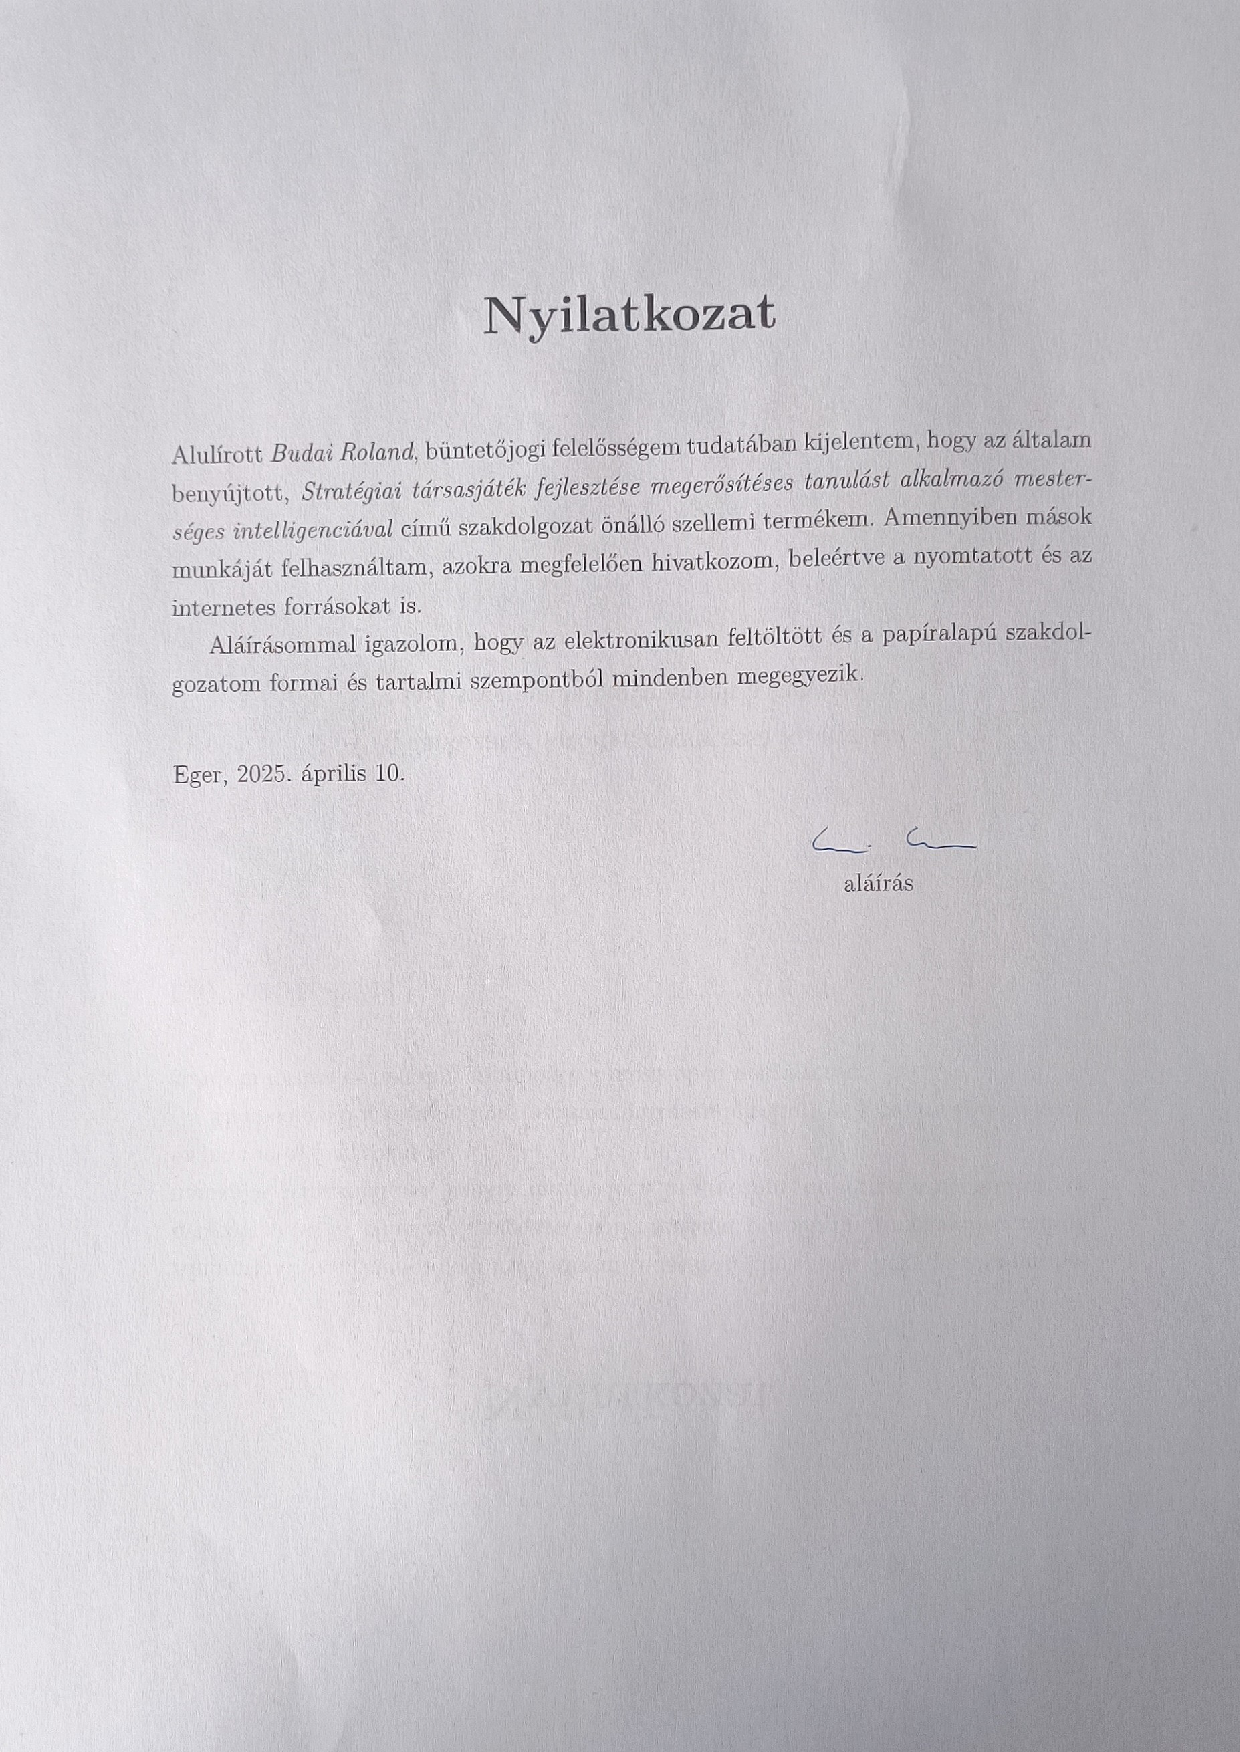
\includepdf{nyilatkozat.pdf}

\end{document}